%%%%%%%%%%%%%%%%%%%%%%%%%%%%%%%%%%%%%%%%%%%%%%%%%%%%%%%%%%%%%%%%%%%%%%%%%%%
% Beamer Presentation
% LaTeX Template
% Version 2.0 (March 8, 2022)
%
% This template originates from:
% https://www.LaTeXTemplates.com
%
% License:
% CC BY-NC-SA 4.0 (https://creativecommons.org/licenses/by-nc-sa/4.0/)
%
%%%%%%%%%%%%%%%%%%%%%%%%%%%%%%%%%%%%%%%%%%%%%%%%%%%%%%%%%%%%%%%%%%%%%%%%%%%
%%%%%%%%%%%%%%%%%%%%%%%%%%%%%%%%%%%%%%%%%%%%%%%%%%%%%%%%%%%%%%%%%%%%%%%%%%%
%
%%%%%%%%%%%%%%%%%%%%%%%%% MADE BY RICARDO CHIN %%%%%%%%%%%%%%%%%%%%%%%%%%%%
%
%%%%%%%%%%%%%%%%%%%%%%%%%%%%%%%%%%%%%%%%%%%%%%%%%%%%%%%%%%%%%%%%%%%%%%%%%%%
%%%%%%%%%%%%%%%%%%%%%%%%%%%%%%%%%%%%%%%%%%%%%%%%%%%%%%%%%%%% December 2023
%
% github.com/roaked 
% ricardochin.com
%                                                          git: MIT License
%----------------------------------------------------------------------------------------
%	PACKAGES AND OTHER DOCUMENT CONFIGURATIONS
%----------------------------------------------------------------------------------------

\documentclass[
	11pt, 
]{beamer}

\graphicspath{{Images/}{./}} 
\usepackage{graphicx}
\usepackage{booktabs} 
\usepackage{tikz}
\usetikzlibrary{shapes.arrows}
% Allows the use of \toprule, \midrule and \bottomrule for better rules in tables


\definecolor{offwhite}{HTML}{F8F8F2}
\definecolor{lightgrey}{HTML}{75715E}
\definecolor{mediumgrey}{HTML}{49483E}
\definecolor{darkgrey}{HTML}{272822}
\definecolor{blue}{HTML}{900C3F}
\definecolor{arrow}{HTML}{900C3F}

\tikzset{
    myarrow/.style={
        draw,
        fill=arrow,
        single arrow,
        minimum height=3.5ex,
        single arrow head extend=1ex
    }
}
\newcommand{\arrowup}{%
\tikz [baseline=-0.5ex]{\node [myarrow,rotate=90] {};}
}
\newcommand{\arrowdown}{%
\tikz [baseline=-1ex]{\node [myarrow,rotate=-90] {};}
}

\usepackage{tcolorbox}
\tcbuselibrary{minted,breakable,xparse,skins}

\definecolor{bg}{gray}{0.95}
\DeclareTCBListing{mintedbox}{O{}m!O{}}{%
  breakable=true,
  listing engine=minted,
  listing only,
  minted language=#2,
  minted style= monokai,
  minted options={%
    linenos,
    gobble=0,
    breaklines=true,
    breakafter=,,
    fontsize=\small,
    numbersep=8pt,
    #1},
  boxsep=0pt,
  left skip=0pt,
  right skip=0pt,
  left=20pt,
  right=0pt,
  top=1pt,
  bottom=1pt,
  arc=5pt,
  leftrule=0pt,
  rightrule=1pt,
  bottomrule=1.5pt,
  toprule=1.5pt,
  colback=darkgrey,
  colframe=blue!70,
  enhanced,
  overlay={%
    \begin{tcbclipinterior}
    \fill[blue!20!white] (frame.south west) rectangle ([xshift=15pt]frame.north west);
    \end{tcbclipinterior}},
  #3}

%----------------------------------------------------------------------------------------
%	SELECT LAYOUT THEME
%----------------------------------------------------------------------------------------

\usetheme{Boadilla} %ok
%\usetheme{CambridgeUS} %red
%\usetheme{Goettingen} % ok
%\usetheme{Singapore} %good
%\usetheme{Szeged} %good

%----------------------------------------------------------------------------------------
%	SELECT COLOR THEME
%----------------------------------------------------------------------------------------


\usecolortheme{seahorse}



%----------------------------------------------------------------------------------------
%	SELECT FONT THEME & FONTS
%----------------------------------------------------------------------------------------

\usefonttheme{default}

%\usepackage{mathptmx} % Use the Times font for serif text
\usepackage{palatino} % Use the Palatino font for serif text
%\usepackage{helvet} % Use the Helvetica font for sans serif text
\usepackage[default]{opensans} % Use the Open Sans font for sans serif text
%\usepackage[default]{FiraSans} % Use the Fira Sans font for sans serif text
%\usepackage[default]{lato} % Use the Lato font for sans serif text

%----------------------------------------------------------------------------------------
%	SELECT INNER THEME
%----------------------------------------------------------------------------------------

%\useinnertheme{default}
\useinnertheme{circles}
%\useinnertheme{rectangles}
%\useinnertheme{rounded}
%\useinnertheme{inmargin}

%----------------------------------------------------------------------------------------
%	SELECT OUTER THEME
%----------------------------------------------------------------------------------------

%\useoutertheme{default}
%\useoutertheme{infolines}
%\useoutertheme{miniframes}
%\useoutertheme{smoothbars}
%\useoutertheme{sidebar}
%\useoutertheme{split}
%\useoutertheme{shadow}
%\useoutertheme{tree}
%\useoutertheme{smoothtree}

%----------------------------------------------------------------------------------
%	PRESENTATION INFORMATION
%----------------------------------------------------------------------------------

\title[Python: Intermediate Fundamentals]{Intermediate Workshop to Python Programming}
\subtitle{Building the Foundation for Coding Success}
\author[Ricardo Chin]{Ricardo Chin}

\begin{document}
\begin{frame}
    \titlepage
    \begin{figure}
        
\includegraphics[width=0.1\linewidth]{5848152fcef1014c0b5e4967}
    \end{figure}
    \frametitle{Workshop Details}
\end{frame}

%----------------------------------------------------------------------------------
%	TABLE OF CONTENTS SLIDE
%----------------------------------------------------------------------------------

\begin{frame}
	\frametitle{Presentation Overview}
	
	\tableofcontents
	%\tableofcontents[pausesections] % Output the table of contents (break sections up across separate slides)
\end{frame}


%%%%%%%%%%%%%%%%%%%%%%%%%%%%%%%%%%%%%%%%%%%%%%%%%%%%%%%%%%%%%%%%%%%%%%%%%%%%%%%

\section{Numeric Data Types} %change
\begin{frame}[fragile]{Data Types: Deeper Dive} %change

\begin{center}
--- Previously in \textsc{Python Programming} ---

\vspace{.25cm}
\arrowdown
\end{center}

\begin{itemize}
    \item \texttt{int}: Whole numbers without decimal points
    \item \texttt{float}: Numbers with decimal points
    \item \texttt{bool}: Represents the truth values \texttt{True} or \texttt{False}
    \item \texttt{NoneType} (\texttt{None}): Represents absence of a value (or null)
    \item \texttt{string}: Ordered sequence of characters 
\end{itemize}

\vspace{.2cm}

\textbf{Collections}
\begin{itemize}
    \item \texttt{list}: Ordered and mutable sequence of elements
    \item \texttt{tuple}: Ordered and immutable sequence of elements
    \item \texttt{dict}: Unordered collection of key-value pairs
\end{itemize}

\end{frame}

%%%%%%%%%%%%%%%%%%%%%%%%%%%%%%%%%%%%%%%%%%%%%%%%%%%%%%%%%%%%%%%%%%%%%%%%%%%%%%%

\begin{frame}[fragile]{NoneType} %change

\textbf{NoneType}
\begin{itemize}
    \item \texttt{None} is a Singleton --- there is only ever a single instance of it inside a running Python program
    \item Multiple variables may refer to that same instance
\end{itemize}

\vspace{.2cm}

\textbf{Comparisons using Keyword \texttt{"is"}}

\vspace{.2cm}

Keyword \texttt{is} checks whether two names refer to the same object

\vspace{.4cm}

\begin{minipage}[t]{0.38\textwidth}
\begin{center}
\begin{mintedbox}{python}
a = [1, 2]
b = a
x = [1, 2]

a == b # True
a is b # True
a == x # True
a is x # False
\end{mintedbox}
\end{center}
\end{minipage}
\hfill
\begin{minipage}[t]{0.55\textwidth}
As \texttt{None} is a singleton, we can check for it via \texttt{is None}

\begin{mintedbox}{python}
if a is None:
    print("a is None")
\end{mintedbox}

\end{minipage}
\end{frame}

%%%%%%%%%%%%%%%%%%%%%%%%%%%%%%%%%%%%%%%%%%%%%%%%%%%%%%%%%%%%%%%%%%%%%%%%%%%%%%%

\begin{frame}[fragile]{BoolType} %change

\textbf{BoolType}
\vspace{.2cm}
\begin{itemize}
    \item The \texttt{bool} type is a built-in data type representing truth values
    \item It has two possible values: \texttt{True} and \texttt{False}
\end{itemize}

\begin{minipage}[t]{0.39\textwidth}
\begin{mintedbox}{python}
a = True
if a:
    print('hello')
\end{mintedbox}
\end{minipage}
\hfill
\begin{minipage}[t]{0.60\textwidth}
\begin{mintedbox}{python}
x, y = 10, 20
is_greater = x > y   # False
if is_greater:
    print("x greater than y")
else:
    print("x not greater than y")
\end{mintedbox}
\end{minipage}

\vspace{.3cm}

Booleans are a subset of integers (subclass of int) where \texttt{True} behaves as 1 and \texttt{False} as 0 in numerical contexts

\centering
\vspace{.4cm}
\texttt{False + True \# 1}

\end{frame}

%%%%%%%%%%%%%%%%%%%%%%%%%%%%%%%%%%%%%%%%%%%%%%%%%%%%%%%%%%%%%%%%%%%%%%%%%%%%%%%

\begin{frame}[fragile]{Numbers} %change

\begin{block}{\textbf{Operations with Numbers}}
    \begin{itemize}
        \item Integer Division: 10 // 3 = 3
        \item Remainder: 10 \% 3 = 1
        \item Exponentiation: 2 ** 3 = 8
    \end{itemize}
    
\end{block}
\vspace{.22cm}
\pause
\begin{center}
    \arrowdown
\end{center}
\vspace{.22cm}

\begin{block}{\textbf{Underscores in Numeric Literals for Enhanced Readibility}}
    \begin{itemize}
        \item Revenue: 1000000000
        \item Revenue: 1\_000\_000\_000
    \end{itemize}
    
\end{block}
    

\end{frame}

%%%%%%%%%%%%%%%%%%%%%%%%%%%%%%%%%%%%%%%%%%%%%%%%%%%%%%%%%%%%%%%%%%%%%%%%%%%%%%%

\begin{frame}[fragile]{Integer Type Representations} %change

\begin{block}{\textbf{Integers}}
\begin{enumerate}
    \item Python supports integers of arbitrary size, allowing representation of very large numbers 

    \item It also supports different numeral systems
    \vspace{.1cm}
    \begin{itemize}
        \item Decimal --- \texttt{a = 42}
        \item Binary ---  \texttt{b = 0b101010}
        \item Octal ---  \texttt{c = 0o52}
        \item Hexadecimal ---  \texttt{d = 0x2a}
        \item Conversion from a string in binary to an integer --- \texttt{e = int('101010', 2)}
    \end{itemize}

\end{enumerate}
\end{block}


\begin{exampleblock}{\textbf{Tip ---} Maximum Size of Integers on the Current System}
\vspace{.05cm}
\begin{mintedbox}{python}   
import sys
print(sys.maxsize)  # Maximum size
\end{mintedbox}
\end{exampleblock}

\end{frame}


%%%%%%%%%%%%%%%%%%%%%%%%%%%%%%%%%%%%%%%%%%%%%%%%%%%%%%%%%%%%%%%%%%%%%%%%%%%%%%%

\begin{frame}[fragile]{Float Type Representations} %change

\begin{block}{\textbf{Integers}}
\begin{enumerate}
    \item Floating-point numbers in Python use 64 bits
        \begin{itemize}
            \item \textbf{Numbering} --- \hspace{.1cm} \texttt{a = .12} \hspace{.1cm} or \hspace{.3cm} \texttt{b = 2.55}
            \item \textbf{Scientific Notation} --- \hspace{.1cm} \texttt{c = 6e23}
            \item \textbf{Special Values} --- \texttt{d = float('nan')}  or  \hspace{.1cm} \texttt{e = float('inf')}
        \end{itemize}


\end{enumerate}
\end{block}

\begin{figure}
    \centering
    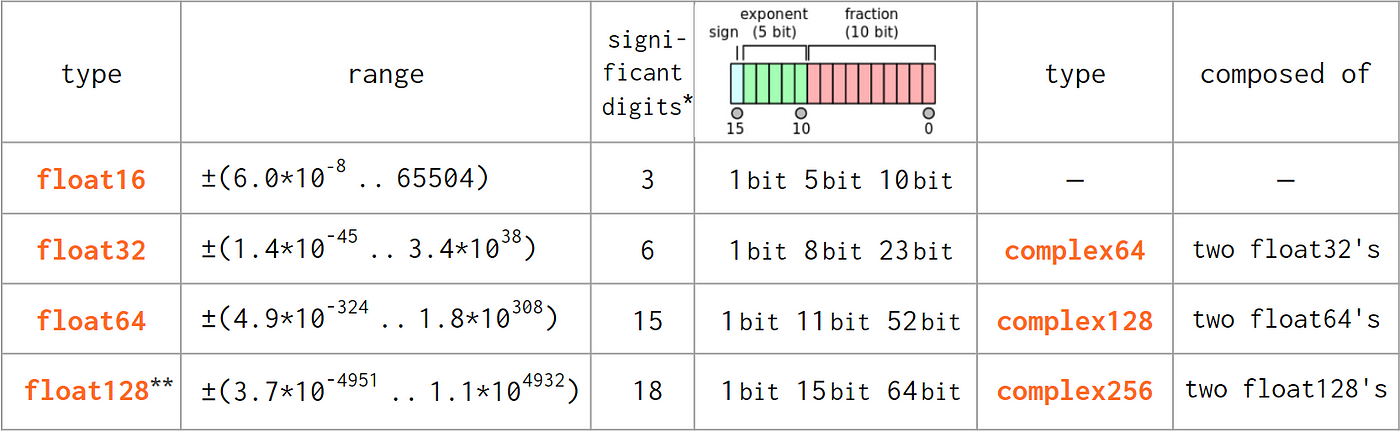
\includegraphics[width = 12cm]{Images/bits.png}
    \caption{Based on IEEE 754 --- Standardized Floating-point Arithmetic}
\end{figure}

\end{frame}

%%%%%%%%%%%%%%%%%%%%%%%%%%%%%%%%%%%%%%%%%%%%%%%%%%%%%%%%%%%%%%%%%%%%%%%%%%%%%%%

\begin{frame}[fragile]{Float Type Representations} %change

\begin{alertblock}{\textbf{Warning!}}
    Floating-point numbers, while versatile, can't perfectly represent all real numbers. This limitation leads to rounding errors, causing some numbers to be approximations rather than precise representations
\end{alertblock}

\pause
\begin{center}
    \arrowdown
\end{center}


In the decimal system:
\begin{enumerate}
    \item Fractions like 1/3 and 1/7 can't be represented exactly
    \item Constant like $\pi$ isn't fully representable without approximation
\end{enumerate}

In binary floats:
\begin{enumerate}
    \item Decimals like 1/2 and 1/10 can't be precisely represented
    \item Fractions like 1/3 and even π suffer from approximation
\end{enumerate}

\end{frame}

%%%%%%%%%%%%%%%%%%%%%%%%%%%%%%%%%%%%%%%%%%%%%%%%%%%%%%%%%%%%%%%%%%%%%%%%%%%%%%%

\begin{frame}[fragile]{Float Rounding Errors} %change

\begin{alertblock}{\textbf{Warning!}}
    As a consequence to not being able to perfectly represent all real numbers, float numbers will lead to rounding error mismatches
\end{alertblock}

\textbf{Example 1 --- Precision Limitations}
\begin{enumerate}
    \item Computing $\pi$ + $\pi$ might yield 6.2 when using decimal numbers with a precision of 2, whereas a more precise result would be 6.3
\end{enumerate}

\textbf{Example 1 --- Arithmetic Precision}
\begin{enumerate}
    \item Simple addition like 0.1 + 0.2 might oddly evaluate to $\approx$ 0.30000000000000004 due to limitations in 64-bit floats
\end{enumerate}
\vspace{.1cm}

\begin{mintedbox}{python}
0.1 + 0.2 == 0.3 # Returns False if float assigned

import math      # tolerance = 1e-09
math.isclose(0.1 + 0.2, 0.3) # Returns True
\end{mintedbox}

\end{frame}


%%%%%%%%%%%%%%%%%%%%%%%%%%%%%%%%%%%%%%%%%%%%%%%%%%%%%%%%%%%%%%%%%%%%%%%%%%%%%%%

\begin{frame}[fragile]{Complex Type and Augmented Assignment} %change

A complex number is a numerical type used to represent numbers that have both a real part and an imaginary part: \texttt{a = 1 + 2j}

\vspace{.1cm}

\textbf{Let us increment the real part \texttt{(1)} of the variable $a$}

\[
a = a + 1 \hspace{.3cm} \texttt{or} \hspace{.3cm} a+= 1
\]

\begin{exampleblock}{\textbf{Augmented Assignment}}
This operation means "add 1 to the current value of $a$ and assign the result back to $a$ 
\end{exampleblock}

\vspace{.12cm}

Calculation:
\[
a = 1 + 2j + 1
\]

Result:
\[
a = 2 + 2j
\]

Other operations include: \hspace{.1cm} \texttt{-=, *=, ...}

\end{frame}

%%%%%%%%%%%%%%%%%%%%%%%%%%%%%%%%%%%%%%%%%%%%%%%%%%%%%%%%%%%%%%%%%%%%%%%%%%%%%%%

\section{Character Encodings}
\begin{frame}{Character Encodings}

Character encodings are used to represent characters in a form that computers can understand and manipulate --- mapping characters to bit sequences

\begin{block}{\textbf{Types of Character Encodings}}
     \begin{enumerate}
         \item ASCII (American Standard Code for Information Interchange)
         \begin{itemize}
             \item Encodes the first 128 Unicode characters using 7 bits, covering basic English characters, digits, and symbols
             \item Represents characters like 'A', '!', '\$', space, and line breaks
         \end{itemize}
         \item Latin1 (ISO 8859-1)
         \begin{itemize}
             \item Extends ASCII to encode the first 256 Unicode characters using 8 bits
             \item Adds additional characters like '$\ddot{a}$ ', '$á$ ', '$\beta$', '$\S$', etc
        
         \end{itemize}
         \item UTF-8, UTF-16, UTF-32
         \begin{itemize}
             \item Encode the entire Unicode character set
             \item UTF-8, a popular encoding, uses variable-width encoding
         \end{itemize}
     \end{enumerate}
\end{block}
    
\end{frame}

%%%%%%%%%%%%%%%%%%%%%%%%%%%%%%%%%%%%%%%%%%%%%%%%%%%%%%%%%%%%%%%%%%%%%%%%%%%%%%%

\begin{frame}{Character Encodings}

Examples in ASCII / Latin1 / UTF-8:

\begin{center}
\vspace{.1cm}
\begin{tabular}{|c|c|}
\hline
Character & Byte Representation \\
\hline
! & 00100001 \\
A & 01000001 \\
Line Feed | Line Break | "\textbackslash{}n" & 00001010 \\
\hline
\end{tabular}
\end{center}

Examples in Latin1:

\begin{center}
\vspace{.1cm}
\renewcommand{\arraystretch}{1.3}
\begin{tabular}{|c|c|}
\hline
Character & Byte Representation \\
\hline
$\ddot{A}$ & 11000100 \\
\hline
\end{tabular}
\end{center}

Examples in UTF-8:

\begin{center}
\vspace{.1cm}
\renewcommand{\arraystretch}{1.3}
\begin{tabular}{|c|c|}
\hline
Character & Byte Representation \\
\hline
$\ddot{A}$ & 11000011 10100100 \\
$\ddot\smile$ & 11110000 10011111 10011001 10000010 \\
\hline
\end{tabular}
\end{center}
    
\end{frame}

%%%%%%%%%%%%%%%%%%%%%%%%%%%%%%%%%%%%%%%%%%%%%%%%%%%%%%%%%%%%%%%%%%%%%%%%%%%%%%%

\begin{frame}{Strings}

Strings represent sequences of Unicode characters, allowing the manipulation and representation of text data

\begin{center}
    \arrowdown
\end{center}

\begin{enumerate}
    \item \textbf{String Literals} --- Representations of strings in Python
    \begin{itemize}
        \item Single quotes: \texttt{a = 'test'}
        \item Double quotes: \texttt{b = "test"}
    \end{itemize}
    \vspace{.3cm}

    \item \textbf{Multi-line String Literals} --- Multi-line representation 
    \texttt{\\
    a = """this\\
    is a multi-line\\
    string literal
    """}
    \vspace{.3cm}
    
    \item \textbf{Escape Sequences} --- \texttt{a = "He said:\textbackslash{}n\textbackslash{}"Hi!\textbackslash{}""} \\
    \textbackslash{}n for line feed or line break!
\end{enumerate}
    
\end{frame}

%%%%%%%%%%%%%%%%%%%%%%%%%%%%%%%%%%%%%%%%%%%%%%%%%%%%%%%%%%%%%%%%%%%%%%%%%%%%%%%

\begin{frame}[fragile]{Strings}

If there is no need to use any escape sequences in a string

\begin{mintedbox}{python}
path = r"C:\documents\course\news.txt"
\end{mintedbox}

Handy when writing directory paths and regular expressions

\begin{exampleblock}{Useful String Methods}
    \begin{itemize}
        \item \texttt{.lower()} and \texttt{.upper()}
        \item \texttt{.startswith(...)} and \texttt{.endswith(".xlsx")}
        \item \texttt{.center(10)} --- centered in 10 chars
        \item \texttt{.ljust(10)} --- left justified or \texttt{.rjust(10)} --- right justified
        \item \texttt{.strip()} --- removes leading and trailing spaces
        \item \texttt{.split(' ')} --- splits a string into a list of substrings
        \item \texttt{' '.join(list)} --- join a list of strings into a single string 
    \end{itemize}
\end{exampleblock}

\end{frame}

%%%%%%%%%%%%%%%%%%%%%%%%%%%%%%%%%%%%%%%%%%%%%%%%%%%%%%%%%%%%%%%%%%%%%%%%%%%%%%%

\begin{frame}[fragile]{String Exercises}

\begin{alertblock}{\textbf{Exercises}}
\begin{enumerate}
    \item Later
\end{enumerate}    
\end{alertblock}

\end{frame}


%%%%%%%%%%%%%%%%%%%%%%%%%%%%%%%%%%%%%%%%%%%%%%%%%%%%%%%%%%%%%%%%%%%%%%%%%%%%%%%

\begin{frame}[fragile]{String Formatting}

String formatting allows for the inclusion of values within strings

\begin{mintedbox}{python}
name = "Ricardo"     
# Concatenation
greeting = "Hello, " + name + "!"

# f-string (formatted string literals)
greeting = f"Hello, {name}!"
\end{mintedbox}

There are other formatting ways which are currently a bit obsolete

\begin{mintedbox}{python}
city, temperature = 'Graz', 5.7    
'weather in %s: %f°C' % (city, temperature)
'weather in {0}: {1}°C'.format(city, temperature)
'weather in {}: {}°C'.format(city, temperature)
'weather in {c}: {t}°C'.format(c=city, t=temperature)
f'weather in {city}: {temperature}°C' # fstring pref
\end{mintedbox}

\end{frame}

%%%%%%%%%%%%%%%%%%%%%%%%%%%%%%%%%%%%%%%%%%%%%%%%%%%%%%%%%%%%%%%%%%%%%%%%%%%%%%%

\begin{frame}[fragile]{Format Specifications}

If we want to specify the format value itself --- ie, \texttt{.4g} or \texttt{.4f}

\begin{mintedbox}{python}
# Four decimal places after the decimal point
print(f"Pi is {math.pi:.4f}") # Output: Pi is 3.1416

# Four significant digits
print(f"Pi is {math.pi:.4g}") # Output: Pi is 3.142
\end{mintedbox}

If we want to specify the sentence alignment

\begin{mintedbox}{python}
first_name, last_name = "Ricardo", "Chin"

# Right-aligned (total width 8 characters)
print(f"{first_name:>8}")  # Output: " Ricardo"
print(f"{last_name:>8}")   # Output: "    Chin"
\end{mintedbox}

\begin{itemize}
    \item \href{https://mkaz.blog/working-with-python/string-formatting/}{String Formatting Reference --- Hyperlink}
\end{itemize}

\end{frame}

%%%%%%%%%%%%%%%%%%%%%%%%%%%%%%%%%%%%%%%%%%%%%%%%%%%%%%%%%%%%%%%%%%%%%%%%%%%%%%%

\begin{frame}[fragile]{Format Specifications}

\begin{alertblock}{\textbf{Exercise}}
\begin{itemize}
    \item Create a program that formats a set of names and associated floating-point numbers representing current spare money, finds longest name, returns the names aligned to the right (longest name) and the spare money with 1 floating point
\end{itemize}
\begin{mintedbox}{python}
# Names
data = [("Ricardo",  12.51), ("Anand",     8.75),
        ("Simon",    15.32), ("Khaled",   10.27)]
\end{mintedbox} 
\end{alertblock}
\pause
\begin{mintedbox}{python}
# Find the length of the longest name
longest_name = max(len(name) for name, _ in data)

# Aligned to longest name and spare money with .1f
for name, value in data:
    print(f"{name:>{longest_name}}{value:.1f}")
\end{mintedbox} 
\end{frame}

%%%%%%%%%%%%%%%%%%%%%%%%%%%%%%%%%%%%%%%%%%%%%%%%%%%%%%%%%%%%%%%%%%%%%%%%%

\begin{frame}[fragile]{Bytes and Hexadecimal Notation}

\textbf{Bytes}

\begin{itemize}
    \item Sequences of integers (8 bits) in the range of 0 to 255
    \item Represent various data types, including images, text, and more
    \item Commonly used with storage media or network responses
\end{itemize}

\textbf{Hexadecimal}
\begin{itemize}
    \item Bytes are often written in hexadecimal notation
    \item Values 0 to 15 represented by digits 0-9 and letters A-F
\end{itemize}
\begin{table}[]
    \centering
    \tiny
    \begin{tabular}{c|c}
        Decimal & Hexadecimal \\ \hline 
        1 &  0x1\\
        9 & 0x9 \\
        10 & 0xa \\
        15 & 0xf \\
        16 & 0x10 \\
        17 & 0x11 \\
        31 & 0x1f \\
        32 & 0x20 \\
    \end{tabular}
\end{table}
\begin{itemize}
    \item Python uses the '0x' prefix to denote hexadecimal literals
\end{itemize}
\end{frame}

%%%%%%%%%%%%%%%%%%%%%%%%%%%%%%%%%%%%%%%%%%%%%%%%%%%%%%%%%%%%%%%%%%%%%%%%%%%%%%%

\begin{frame}[fragile]{Bytes and String Encodings}

\textbf{Creating Bytes from Lists}

\begin{mintedbox}{python}
a = bytes([0, 64, 112, 160, 255])
b = bytes([0, 0x40, 0x70, 0xa0, 0xff])
print(bytes([0x00, 0x40, 0x70, 0xa0, 0xff])) # 'a'
\end{mintedbox}

\begin{itemize}
    \item Illustrates creating bytes from a list of numbers
    \item Hexadecimal values can also be used directly
\end{itemize}

\textbf{Creating Bytes from Byte Literal Strings}

\begin{mintedbox}{python}
c = b"\x00\x40\x70\xa0\xff"
\end{mintedbox}

\begin{itemize}
    \item 'b' prefix indicates a byte string
    \item Bytes usually hold encoded text, so we can do: \texttt{'ä'.encode('utf-8')} and \texttt{b'\xc3\xa4'.decode('utf-8')}
    \item Also possible to represent it with ASCII characters
\end{itemize}



\end{frame}

%%%%%%%%%%%%%%%%%%%%%%%%%%%%%%%%%%%%%%%%%%%%%%%%%%%%%%%%%%%%%%%%%%%%%%%%%%%%%%%

\section{Data Structures}
\begin{frame}[fragile]{Lists}

\textbf{Lists}
\begin{itemize}
    \item Dynamic arrays for storing sequences of objects
    \item Versatile and mutable
    \item Ideal for homogenous entries of the same type and structure
\end{itemize}

\begin{mintedbox}{python}
primes = [2, 3, 5, 7, 11]
users = ["Ricardo", "Anand", "Blazhe"]
\end{mintedbox} 

\textbf{List Operations}

\begin{itemize}
    \item Indexing
\end{itemize}
\begin{mintedbox}{python}
primes[0] # returns 2 
primes[-1] # returns last element of the list -> 11
\end{mintedbox} 
\begin{itemize}
    \item Accessing multiple elements (sublists)
\end{itemize}
 \begin{mintedbox}{python}
primes[1:4] # returns [3, 5, 7]
\end{mintedbox}    
\end{frame}

%%%%%%%%%%%%%%%%%%%%%%%%%%%%%%%%%%%%%%%%%%%%%%%%%%%%%%%%%%%%%%%%%%%%%%%%%%%%%%%

%%%%%%%%%%%%%%%%%%%%%%%%%%%%%%%%%%%%%%%%%%%%%%%%%%%%%%%%%%%%%%%%%%%%%%%%%%%%%%%

\begin{frame}[fragile]{Lists}

\begin{itemize}
    \item Modifying lists (append, insert, pop)
\end{itemize}
\begin{mintedbox}{python}
primes.append(13) # add 13 to the list primes
primes.insert(0, "Khaled") # Khaled to beginning
primes.pop() # pops last element of the list
primes.pop(0) # pops element at index 0
\end{mintedbox} 
\begin{itemize}
    \item Characteristics of the list
\end{itemize}
\begin{mintedbox}{python}
len(primes) # returns the size of the list
max(primes) # returns the max value of the list
min(primes) # returns the min value of the list
\end{mintedbox}   
\begin{itemize}
    \item Sorting lists
\end{itemize}
\begin{mintedbox}{python}
primes.sort() # increasing, alphabet for strings
primes.sort(reverse = True) # sorts decreasingly
primes.sort(key = len) # sorts by length
\end{mintedbox}      
\end{frame}

%%%%%%%%%%%%%%%%%%%%%%%%%%%%%%%%%%%%%%%%%%%%%%%%%%%%%%%%%%%%%%%%%%%%%%%%%%%%%%%

\begin{frame}[fragile]{Lists}
\begin{itemize}
    \item Iterating through lists
\begin{mintedbox}{python}
for prime in primes:
    print(prime)
\end{mintedbox}    
    \item Conditionals in lists
\begin{mintedbox}{python}
if "Ricardo" in users:
    print("Ricardo is here.")
\end{mintedbox}
\end{itemize}
\textbf{Example:}

\begin{mintedbox}{python}
users.sort(key = len)

def count_a(s):
    return s.count("a")
    
users.sort(key=count_a)
\end{mintedbox}
\end{frame}

%%%%%%%%%%%%%%%%%%%%%%%%%%%%%%%%%%%%%%%%%%%%%%%%%%%%%%%%%%%%%%%%%%%%%%%%%%%%%%%

\begin{frame}[fragile]{List Exercises}

\begin{alertblock}{\textbf{Exercises}}
\begin{itemize}
    \item Create a list of your favorite colors\\
        Print the length of the list\\
        Access and print the first and last elements of the list\\

    \item Create a list of characters from 'a' to 'e' \\
        Print a slice of the list containing elements 'b' and 'c' \\
        Modify the original list to replace 'c' with 'z' and print it \\

    \item More...
\end{itemize}

\end{alertblock}

\end{frame}

%%%%%%%%%%%%%%%%%%%%%%%%%%%%%%%%%%%%%%%%%%%%%%%%%%%%%%%%%%%%%%%%%%%%%%%%%%%%%%%

\begin{frame}[fragile]{Tuples}

\textbf{Tuples}

\begin{itemize}
    \item Lightweight and immutable sequences of objects
    \item Entries separated by commas, typically surrounded by round brackets
    \item Commonly used for grouping related data
\end{itemize}

\begin{mintedbox}{python}
single_value = ('Ricardo', ) # or
single_value = 'Ricardo', # notice the comma
values = ('Ricardo', 'Chin') # or
values = 'Ricardo', 'Chin'
\end{mintedbox}

\begin{itemize}
    \item Elements in a tuple can be accessed using indexing
    \item \texttt{values[0]} returns 'Ricardo'
\end{itemize}

\begin{mintedbox}{python}
first_name, last_name = two_values # var to tuple
first_name, last_name = last_name, first_name
\end{mintedbox}

\end{frame}

%%%%%%%%%%%%%%%%%%%%%%%%%%%%%%%%%%%%%%%%%%%%%%%%%%%%%%%%%%%%%%%%%%%%%%%%%%%%%%%

\begin{frame}[fragile]{Dictionaries}

\textbf{Dictionaries}

\begin{itemize}
    \item Mappings of keys to values
    \item Example dictionary representing my information
\end{itemize}

\begin{mintedbox}{python}
individual = {
    "first_name": "Ricardo",
    "last_name": "Chin",
    "nationality": "Portuguese",
    "birth_year": 1996
}
\end{mintedbox}

\begin{itemize}
    \item Elements in a dictionary can be accessed using the keys
\end{itemize}

\begin{mintedbox}{python}
individual["first_name"]  # return "Ricardo"
\end{mintedbox}

\end{frame}

%%%%%%%%%%%%%%%%%%%%%%%%%%%%%%%%%%%%%%%%%%%%%%%%%%%%%%%%%%%%%%%%%%%%%%%%%%%%%%%

\begin{frame}[fragile]{Dictionaries}

\textbf{Iterations Over Dictionaries}

\begin{mintedbox}{python}
for key in individual:
    print(key)
\end{mintedbox}

\begin{itemize}
    \item Keys: "first\_name", "last\_name", "nationality", "birth\_year"
\end{itemize}

\begin{exampleblock}{\textbf{Tip}}
    Dictionary keys are maintained in insertion order
\end{exampleblock}

\textbf{Iterations Over Key-Value Pairs}
\begin{mintedbox}{python}
for key, value in person.items():
    print(f'{key}, {value}')
\end{mintedbox}

\begin{itemize}
    \item Shows how to iterate over key-value pairs in dictionaries
    \item Utilizes the \texttt{items()} method for iteration
\end{itemize}
\end{frame}

%%%%%%%%%%%%%%%%%%%%%%%%%%%%%%%%%%%%%%%%%%%%%%%%%%%%%%%%%%%%%%%%%%%%%%%%%%%%%%%

\begin{frame}[fragile]{Dictionaries}

\textbf{Operations on Dictionaries}

\begin{mintedbox}{python}
d = {0: 'Ricardo', 1: 'Anand', 2: 'Blazhe'}
d[2] # value of key 2
d[2] = 'Thomas'
d[3]  # raises KeyError
d.get(3)  # returns None (similar to above, but safe)
d.setdefault(2, 'n')
d.setdefault(3, 'n')

d.keys() # get keys from dictionary
d.items() # get key-value pairs from dictionary
d1.update(d2) # overwrites if key is existing already
\end{mintedbox}

\begin{itemize}
    \item Using \texttt{get()} and \texttt{setdefault()} for safe key retrieval
    \item Retrieving keys and items (key-value pairs)
    \item Updating dictionaries using \texttt{update(d)} or \texttt{extend(value)}
\end{itemize}


\end{frame}

%%%%%%%%%%%%%%%%%%%%%%%%%%%%%%%%%%%%%%%%%%%%%%%%%%%%%%%%%%%%%%%%%%%%%%%%

\begin{frame}[fragile]{Dictionary Exercises}

\begin{alertblock}{\textbf{Exercises}}
\begin{itemize}
    \item Later...
\end{itemize}

\end{alertblock}
\end{frame}

%%%%%%%%%%%%%%%%%%%%%%%%%%%%%%%%%%%%%%%%%%%%%%%%%%%%%%%%%%%%%%%%%%%%%%%%%%%%%%%

\section{Object Oriented Programming}
\begin{frame}[fragile]{Object Oriented Programming (OOP)}

\begin{block}{\textbf{Introduction to OOP}}
    \begin{itemize}
        \item Python follows the OOP paradigm
        \item The mantra: "Everything is an object.
    \end{itemize}
\end{block}

\textbf{Examples:}

\begin{mintedbox}{python}
# Example 1: Integer
a = 20

# Example 2: Method Call on Integer
bytes_representation = a.to_bytes(1, "big")

# Example 3: Method Call on String
uppercase_hello = "hello".upper()
\end{mintedbox}

The integer \texttt{a}, the method \texttt{to\_bytes()}, and the string method \texttt{upper()}


\end{frame}

%%%%%%%%%%%%%%%%%%%%%%%%%%%%%%%%%%%%%%%%%%%%%%%%%%%%%%%%%%%%%%%%%%%%%%%%%%%%%%%

\begin{frame}[fragile]{Types and Instances}

\begin{itemize}
    \item Everything is an object and each object has a type
\end{itemize}

\begin{mintedbox}{python}
message = "hello"
\end{mintedbox}

\begin{itemize}
    \item This line creates a variable message and assigns it the value "hello". For terminology reasons, "hello" is an instance of the string type \texttt{str}
\end{itemize}

\begin{mintedbox}{python}
type(message)
isinstance(message, str)
\end{mintedbox}

\begin{itemize}
    \item \texttt{type()} returns the type of the object
    \item \texttt{isinstance()} checks if the object is an instance of a particular type
    \item the outcome is a Boolean returning \texttt{True} if message is an instance of a \texttt{str} type, otherwise \texttt{False}
\end{itemize}


\end{frame}

%%%%%%%%%%%%%%%%%%%%%%%%%%%%%%%%%%%%%%%%%%%%%%%%%%%%%%%%%%%%%%%%%%%%%%%%%%%%%%%

\begin{frame}[fragile]{Classes}

\begin{itemize}
    \item Classes are defined by the keyword \texttt{Class}
    \item The definition of class usually encompasses:
    \begin{enumerate}
        \item \textbf{Attributes} --- Properties of a class where data is stored
        \item \textbf{Methods} --- Specific behaviours or functionalities of that class
        \item \textbf{Constructor} --- \texttt{The \_\_init\_\_} method is a special method. It is called when an object is created and is used to initialize the object's attributes
    \end{enumerate}
\end{itemize}

\begin{mintedbox}{python}
class BankAccount(object):
    def __init__(self, account_number, balance):
        self.account_number = account_number
        self.balance = balance
    
    def deposit(self, amount):
        # Method for depositing money
    
    def withdraw(self, amount):
        # Method for withdrawing money
\end{mintedbox}

\end{frame}

%%%%%%%%%%%%%%%%%%%%%%%%%%%%%%%%%%%%%%%%%%%%%%%%%%%%%%%%%%%%%%%%%%%%%%%%%%%%%%%

\begin{frame}[fragile]{Classes}
\tiny
\begin{mintedbox}{python}
class BankAccount(object):
    def __init__(self, account_number, balance):
        self.account_number = account_number
        self.balance = balance

    def deposit(self, amount): # Deposit amount 
        self.balance += amount
        print(f"New balance: {self.balance}€")

    def withdraw(self, amount): # Withdraw amount
        if amount <= self.balance:
            self.balance -= amount
            print(f"New balance: {self.balance}€")
        else:
            print("Insufficient funds.")

    def check_balance(self): # Current balance
        print(f"Current balance: {self.balance}€")
\end{mintedbox}
\end{frame}

%%%%%%%%%%%%%%%%%%%%%%%%%%%%%%%%%%%%%%%%%%%%%%%%%%%%%%%%%%%%%%%%%%%%%%%%%%%%%%%

\begin{frame}[fragile]{Classes}
\begin{mintedbox}{python}
# Create an instance of the BankAccount class
my_account = BankAccount("100_000", 1000)
# Use the methods of the BankAccount class
my_account.check_balance()  # Current balance: 1000€
my_account.deposit(500)     # New balance: 1500€
my_account.withdraw(200)    # New balance: 1300€
my_account.withdraw(1500)   # Insufficient funds. 
my_account.check_balance()  # Current balance: 1300€
\end{mintedbox}

\begin{itemize}
    \item The constructor \texttt{\_\_init\_\_} initializes an object with attributes
\end{itemize}

\begin{alertblock}{\textbf{Warning!}}
    \begin{itemize}
        \item The double underscore in the constructor \texttt{\_\_init\_\_} indicates that this method is intended for internal use within the class and should not be accessed or modified directly from outside the class. This is called \textbf{mangling}
    \end{itemize}
\end{alertblock}

\end{frame}

%%%%%%%%%%%%%%%%%%%%%%%%%%%%%%%%%%%%%%%%%%%%%%%%%%%%%%%%%%%%%%%%%%%%%%%%%%%%%%%

\begin{frame}[fragile]{Classes}

\begin{itemize}
    \item We can instance private attributes and methods
\end{itemize}
\begin{mintedbox}{python}
class BankAccount:
    def __init__(self, account_number, balance):
        self.__account_number = account_number  
        self.__balance = balance # Private attrivyte             

    def __validate_withdrawal(self, amount): 
        """Validate if withdrawal is possible."""
        return amount <= self.__balance
\end{mintedbox}

\begin{itemize}
    \item Attempting to access these directly from outside the class using name mangling is technically possible but not recommended
\end{itemize}

\begin{mintedbox}{python}
print(my_account._BankAccount__account_number) 
my_account._BankAccount__validate_withdrawal(200)
\end{mintedbox}

\end{frame}

%%%%%%%%%%%%%%%%%%%%%%%%%%%%%%%%%%%%%%%%%%%%%%%%%%%%%%%%%%%%%%%%%%%%%%%%%%%%%%%

\begin{frame}[fragile]{Classes}

\begin{alertblock}{\textbf{Exercise}}
\begin{itemize}
    \item Class \texttt{Rectangle} with attributes length and width. Add methods \texttt{calculate\_area()} and \texttt{calculate\_perimeter()} to compute the area and perimeter of the rectangle
    \vspace{.1cm}

    \item Class \texttt{Circle} with attribute radius. Add methods \texttt{calculate\_area()} and \texttt{calculate\_circumference()} to compute the area and circumference of the circle
    \vspace{.1cm}

    \item Class \texttt{Student} with attributes name, age, and grades (a list of grades). Add methods \texttt{add\_grade()} to add a grade to the list and \texttt{average\_grade()} to calculate and return the average
    \vspace{.1cm}

    \item Class \texttt{Playlist}  with attributes name and songs (a list of song objects). Add methods \texttt{add\_song(song\_title)}, \texttt{remove\_song(song\_title)}, and \texttt{display\_songs()}
\end{itemize}

\end{alertblock}

\end{frame}

%%%%%%%%%%%%%%%%%%%%%%%%%%%%%%%%%%%%%%%%%%%%%%%%%%%%%%%%%%%%%%%%%%%%%%%%%%%%%%%

\begin{frame}[fragile]{Inheritance}

\begin{block}{\textbf{What is this fancy word: Inheritance?}}
It is a mechanism in OOP where a new class is created by inheriting attributes and behaviours from an existing class. The subclass automatically gains the methods and attributes of the superclass
\end{block}
\begin{enumerate}
    \item \textbf{New class} --- \texttt{superclass/base class}
    \item \textbf{Existing class} --- \texttt{subclass/derived class}
\end{enumerate}

\begin{mintedbox}{python}
class User(object):
    def __init__(self, username):
        self.username = username
        
class AdminUser(User): # inherited attributes from User
    def __init__(self, username, admin_level):
        super().__init__(username)
        self.admin_level = admin_level
\end{mintedbox}
\end{frame}


%%%%%%%%%%%%%%%%%%%%%%%%%%%%%%%%%%%%%%%%%%%%%%%%%%%%%%%%%%%%%%%%%%%%%%%%%%%%%%%

\begin{frame}[fragile]{Inheritance}

Inheritance is commonly used in defining database models --- example in a popular web framework \texttt{Django}  

\begin{mintedbox}{python}
from django.db import models

class Employee(models.Model):
    name = models.CharField(max_length=50)
    position = models.CharField(max_length=50)
    salary = models.DecimalField(max_digits=10, decimal_places=2)

class RegularEmployee(Employee):
    department = models.CharField(max_length=50)

class Manager(Employee):
    department_mgmt = models.CharField(max_length=50)
    team_size = models.PositiveIntegerField()
\end{mintedbox}
\end{frame}

%%%%%%%%%%%%%%%%%%%%%%%%%%%%%%%%%%%%%%%%%%%%%%%%%%%%%%%%%%%%%%%%%%%%%%%%%%%%%%%

\begin{frame}[fragile]{Inheritance}

\begin{mintedbox}{python}
# Creating instances of RegularEmployee and Manager
...

# Saving instances to the Django database
regular_employee.save()
manager.save()

# Querying the database
all_employees = Employee.objects.all()
regular_employees = RegularEmployee.objects.all()
managers = Manager.objects.all()

# Accessing fields
print(regular_employee.department)
print(manager.department_managed)
print(manager.team_size)
\end{mintedbox}
\end{frame}

%%%%%%%%%%%%%%%%%%%%%%%%%%%%%%%%%%%%%%%%%%%%%%%%%%%%%%%%%%%%%%%%%%%%%%%%%%%%%%%

\begin{frame}[fragile]{Composition}
\begin{block}{\textbf{Composition?}}
Composition is an alternative to inheritance. It involves creating objects from other classes within a class, allowing for more flexibility and avoiding the pitfalls of deep class hierarchies
\end{block}


\begin{mintedbox}{python}
class TicTacToeGame(object):
    def __init__(self):
        # Game logic implementation

class GameGUI(object):
    def __init__(self):
        self.game = TicTacToeGame()
        # GUI implementation using TicTacToeGame
\end{mintedbox}

\begin{itemize}
    \item  GameGUI uses composition by having an instance of TicTacToeGame within it. This way, it can access and use the functionality of TicTacToeGame 
\end{itemize}

\end{frame}

%%%%%%%%%%%%%%%%%%%%%%%%%%%%%%%%%%%%%%%%%%%%%%%%%%%%%%%%%%%%%%%%%%%%%%%%%%%%%%%


\begin{frame}[fragile]{Composition}
\begin{block}{\textbf{Composition?}}
Composition is an alternative to inheritance. It involves creating objects from other classes within a class, allowing for more flexibility and avoiding the pitfalls of deep class hierarchies
\end{block}


\begin{mintedbox}{python}
class TicTacToeGame(object):
    def __init__(self):
        # Game logic implementation

class GameGUI(object):
    def __init__(self):
        self.game = TicTacToeGame()
        # GUI implementation using TicTacToeGame
\end{mintedbox}

\begin{itemize}
    \item  GameGUI uses composition by having an instance of TicTacToeGame within it. This way, it can access and use the functionality of TicTacToeGame 
\end{itemize}

\end{frame}

%%%%%%%%%%%%%%%%%%%%%%%%%%%%%%%%%%%%%%%%%%%%%%%%%%%%%%%%%%%%%%%%%%%%%%%%%%%%%%%


\begin{frame}[fragile]{Docstrings}
These OOP concepts can drastically decrease readibility --- \textbf{This is why docstrings are useful:}
\vspace{.05cm}
\begin{enumerate}
    \item They provide documentation for functions, classes, and modules describing purpose, usage, and behaviour of the code
    \item Placed at the beginning of the function, class, or module
\end{enumerate}

\begin{mintedbox}{python}
def fib(n):
"""Compute the n-th Fibonacci number.

Parameters:
- n (int): A nonnegative integer.

Returns:
int: The n-th Fibonacci number."""
# Function implementation...
\end{mintedbox}

\underline{Further info}: \texttt{help()} function or accessing the \texttt{\_\_doc\_\_} attribute

\end{frame}

%%%%%%%%%%%%%%%%%%%%%%%%%%%%%%%%%%%%%%%%%%%%%%%%%%%%%%%%%%%%%%%%%%%%%%%%%%%%%%%

\section{Control Structures}
\begin{frame}[fragile]{Control Structures}
Control structures are essential components in programming languages that enable the control flow of a program

\begin{block}{\textbf{Control Structures}}
\begin{itemize}
\item if ... else ...
\item loops
\begin{itemize}
    \item while
    \item for ... in ...
    \item for ... in range()
\end{itemize}
\item try ... except ... finally
\end{itemize}
\end{block}

The structure is usually pretty straightforward

\begin{mintedbox}{python}
for i in range(5):
print(i)
\end{mintedbox}
\end{frame}

%%%%%%%%%%%%%%%%%%%%%%%%%%%%%%%%%%%%%%%%%%%%%%%%%%%%%%%%%%%%%%%%%%%%%%%%%%%%%%%

\begin{frame}[fragile]{If Statements}
\footnotesize
Previously we saw conditions for \texttt{if} and \texttt{while} where we usually used expressions that evaluate to boolean values \texttt{(if a == b)}

\begin{center}
    \arrowdown
\end{center}
Any value can be used in a condition as most values are considered "truthy"

\begin{mintedbox}{python}
name = input("Enter your name: ")
if name:
    print(f"Hello, {name}!")
else:
    print("Empty.")
\end{mintedbox}

\begin{center}
    \arrowdown
\end{center}
\begin{mintedbox}{python}
print(f"Hello, {name}!") if name else print("Empty.")
\end{mintedbox}
\begin{minipage}{0.505\textwidth}
\begin{mintedbox}{python}
13 <= age and age <= 19
\end{mintedbox}
\end{minipage}
\hfill
\begin{minipage}{0.485\textwidth}
\begin{mintedbox}{python}
13 <= age <= 19
\end{mintedbox}
\end{minipage}

\end{frame}

%%%%%%%%%%%%%%%%%%%%%%%%%%%%%%%%%%%%%%%%%%%%%%%%%%%%%%%%%%%%%%%%%%%%%%%%%%%%%%%

\begin{frame}[fragile]{For Loops}

\textbf{Recap:} Tuple unpacking allows to assign multiple variables at once when iterating over a sequence

\begin{itemize}
    \item \texttt{enumerate()} is a built-in function that returns an iterator of tuples containing indices and values from a list
\end{itemize}

\begin{mintedbox}{python}
names = ['Ricardo', 'Anand', 'Khaled']

for i, name in enumerate(names):
print(f'{i}: {name}')
\end{mintedbox}

Enumerate returns a data structure that behaves like this list:

\begin{mintedbox}{python}
0: Ricardo
1: Anand
2: Khaled
\end{mintedbox}

\begin{itemize}
    \item \texttt{enumerate()} generates pairs of index and value, allowing to iterate over both simultaneously
\end{itemize}

\end{frame}

%%%%%%%%%%%%%%%%%%%%%%%%%%%%%%%%%%%%%%%%%%%%%%%%%%%%%%%%%%%%%%%%%%%%%%%%%%%%%%%

\begin{frame}[fragile]{Nested For Loops}

\begin{itemize}
    \item \texttt{os.walk()} is used to iterate over all files and subdirectories in a specified directory. We can also nest \texttt{for} loops for going through all the files in the directories
\end{itemize}

\begin{mintedbox}{python}
import os

for directory, dirs, files in os.walk("C:\\"): # all
    for file in files: # Each file in the directory
        if not file.endswith(".xlsx"): # Not excel?
            continue # We skip non-excel files
        
        # Process text files
        file_path = os.path.join(directory, file)
        print(f"Processing: {file_path}")
\end{mintedbox}

\begin{itemize}
    \item \texttt{continue} statement skips the processing for non-xlsx files
\end{itemize}

\end{frame}

%%%%%%%%%%%%%%%%%%%%%%%%%%%%%%%%%%%%%%%%%%%%%%%%%%%%%%%%%%%%%%%%%%%%%%%%%%%%%%%

\begin{frame}[fragile]{List Comprehensions}

List comprehensions provide a concise way to create lists based on existing lists, allowing for transformations and filtering

\begin{mintedbox}{python}
names = ["Ricardo", "Anand", "Khaled"]

uppercase_names = [name.upper() for name in names]
\end{mintedbox}
\begin{mintedbox}{python} 
# Results
["RICARDO", "ANAND", "KHALED"]
\end{mintedbox}

Another example:

\begin{mintedbox}{python}
amounts = [10, -7, 8, 19, -2]

positive_amounts = [amount for amount in amounts if amount > 0]
\end{mintedbox}

This creates a new list \texttt{positive\_amounts} containing only the positive values from the original list \texttt{amounts}

\end{frame}

%%%%%%%%%%%%%%%%%%%%%%%%%%%%%%%%%%%%%%%%%%%%%%%%%%%%%%%%%%%%%%%%%%%%%%%%%%%%%%%

\begin{frame}[fragile]{Dictionary Comprehensions}

Dictionary comprehensions are expressions followed by a \texttt{for} clause inside curly braces {}, and optionally, one or more \texttt{if} clauses

\begin{mintedbox}{python}
{key_exp: value_exp for item in iterable if condition}
\end{mintedbox}

Where an iterable (list, tuple, etc.) contains various items

\begin{mintedbox}{python}
numbers = [1, 2, 3, 4, 5] # Square of numbers
squares = {num: num**2 for num in numbers}
\end{mintedbox}

\begin{mintedbox}{python}
grades = {'Alice': 90, 'Bob': 85, 'Charlie': 92} 
adjusted_grades = {name: grade + 5 for name, grade in grades.items()}
\end{mintedbox}

\end{frame}

%%%%%%%%%%%%%%%%%%%%%%%%%%%%%%%%%%%%%%%%%%%%%%%%%%%%%%%%%%%%%%%%%%%%%%%%%%%%%%%

\begin{frame}[fragile]{Comprehensions}

\begin{alertblock}{\textbf{Exercises}}
    \begin{itemize}
        \item ...later...
    \end{itemize}
\end{alertblock}
\end{frame}


%%%%%%%%%%%%%%%%%%%%%%%%%%%%%%%%%%%%%%%%%%%%%%%%%%%%%%%%%%%%%%%%%%%%%%%%%%%%%%%

\begin{frame}[fragile]{Exception Handling}

Exception handling allows us to manage errors gracefully

\begin{mintedbox}{python}
def divide(a, b):
    try:
        if b == 0:
            raise ValueError("Cannot divide by zero")
        result = a / b
        print(f"The result is: {result}")
    except ValueError as ve:
        print(f"Error: {ve}")
    finally:
        print("This will be executed no matter what")

divide(10, 0) # Try other values
\end{mintedbox}

\begin{enumerate}
    \item The \texttt{try} block attempts to execute the division operation
    \item If a \texttt{ValueError} is raised (due to division by zero), the \texttt{except} block catches it and prints an error message
\end{enumerate}

\end{frame}

%%%%%%%%%%%%%%%%%%%%%%%%%%%%%%%%%%%%%%%%%%%%%%%%%%%%%%%%%%%%%%%%%%%%%%%%%%%%%%%

\section{Modules}
\begin{frame}[fragile]{Module Name and Entrypoint}

....

\end{frame}

%%%%%%%%%%%%%%%%%%%%%%%%%%%%%%%%%%%%%%%%%%%%%%%%%%%%%%%%%%%%%%%%%%%%%%%%%%%%%%%

\begin{frame}[fragile]{Virtual Environments}

....

\end{frame}

%%%%%%%%%%%%%%%%%%%%%%%%%%%%%%%%%%%%%%%%%%%%%%%%%%%%%%%%%%%%%%%%%%%%%%%%%%%%%%%


\begin{frame}[fragile]{Arbitrary Number of Arguments (Args / Kwargs)}

....

\end{frame}

%%%%%%%%%%%%%%%%%%%%%%%%%%%%%%%%%%%%%%%%%%%%%%%%%%%%%%%%%%%%%%%%%%%%%%%%%%%%%%%


\begin{frame}[fragile]{Global and Local Scope}

....

\end{frame}


%%%%%%%%%%%%%%%%%%%%%%%%%%%%%%%%%%%%%%%%%%%%%%%%%%%%%%%%%%%%%%%%%%%%%%%%%%%%%%%

\section{Interesting References}
\begin{frame}[fragile]{Interesting References}
\begin{exampleblock}{\textbf{Books}}
    
\begin{itemize}


\item \href{https://automatetheboringstuff.com/}{Automate the Boring Stuff with Python by Al Sweigart}

\item \href{http://greenteapress.com/thinkpython2/thinkpython2.pdf}{Think Python, 2nd Edition by Allen B. Downey}

\item \href{https://www.py4e.com/book.php}{Python for Everybody by Dr. Charles Severance}

\end{itemize}
\end{exampleblock}

\begin{exampleblock}{\textbf{Online Courses and Tutorials}}

\begin{itemize}

\item \href{https://mkaz.blog/working-with-python/string-formatting/}{String Formatting}

\item \href{https://www.codecademy.com/learn/learn-python-3}{Codecademy - Beginner Course}

\item \href{https://learnxinyminutes.com/docs/python/}{Learn X in Y Minutes - Python}

\item \href{https://ehmatthes.github.io/pcc_2e/cheat_sheets/cheat_sheets/}{Python Cheat Sheets by Eric Matthes}
\end{itemize}
\end{exampleblock}
\end{frame}


%%%%%%%%%%%%%%%%%%%%%%%%%%%%%%%%%%%%%%%%%%%%%%%%%%%%%%%%%%%%%%%%%%%%%%%%%%%%%%%

\begin{frame}[fragile]{The End}

\centering

\Huge Thank you!

\end{frame}


%------------------------------------------------

% \subsection{Columns}

% \begin{frame}
% 	\frametitle{Multiple Columns}
% 	\framesubtitle{Subtitle} % Optional subtitle
	
% 	\begin{columns}[c] % The "c" option specifies centered vertical alignment while the "t" option is used for top vertical alignment
% 		\begin{column}{0.45\textwidth} % Left column width
% 			\textbf{Heading}
% 			\begin{enumerate}
% 				\item Statement
% 				\item Explanation
% 				\item Example
% 			\end{enumerate}
% 		\end{column}
% 		\begin{column}{0.5\textwidth} % Right column width
% 			Lorem ipsum dolor sit amet, consectetur adipiscing elit. Integer lectus nisl, ultricies in feugiat rutrum, porttitor sit amet augue. Aliquam ut tortor mauris. Sed volutpat ante purus, quis accumsan dolor.
% 		\end{column}
% 	\end{columns}
% \end{frame}

\end{document} 
